\documentclass[crop,tikz]{standalone}
\tikzstyle{bag} = [align=center]
\usetikzlibrary{positioning}
\usetikzlibrary{arrows.meta}

\begin{document}
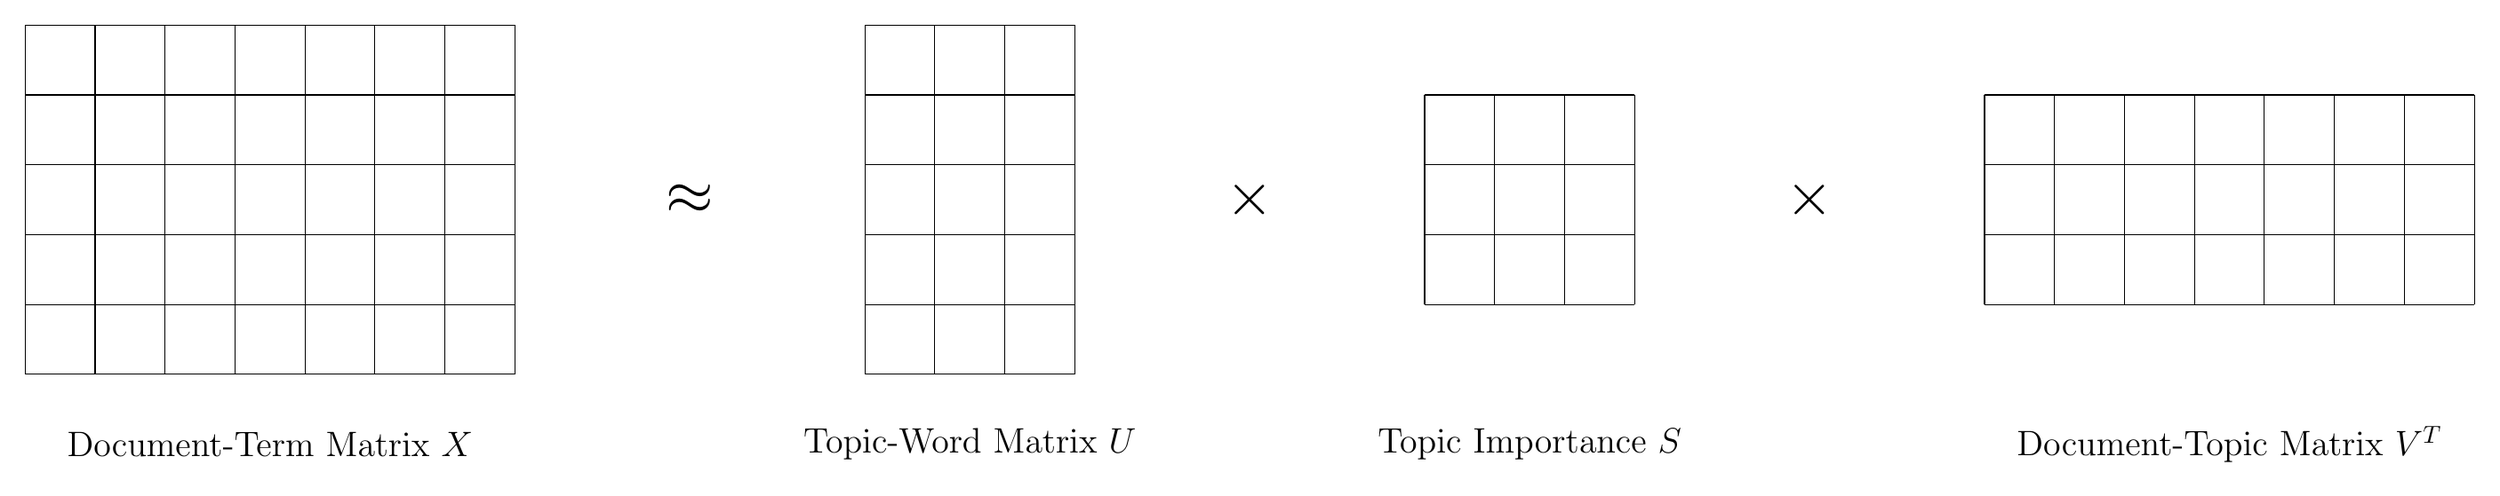
\begin{tikzpicture}[grow=right]

    \foreach \x in {0,...,7}
        \foreach \y in {0,...,5} {
            \draw (\x,0) -- (\x,\y);
            \draw (0,\y) -- (\x,\y);
        }

    \node at (3.5,-1) {\Large Document-Term Matrix $X$};
    \node at (9.5,2.5) {\Huge $\approx$};

    \def\offset{10}
    \foreach \x in {2,...,5}
        \foreach \y in {0,...,5} {
                \draw (\offset+2,\y) -- (\offset+\x,\y);
                \draw (\offset+\x,0) -- (\offset+\x,\y);
        }

    \node at (\offset+3.5,-1) {\Large Topic-Word Matrix $U$};
    \node at (\offset+7.5,2.5) {\Huge $\times$};

    \def\offset{20}
    \foreach \x in {0,...,3}
        \foreach \y in {1,...,4} {
                \draw (\offset,\y) -- (\offset+\x,\y);
                \draw (\offset+\x,1) -- (\offset+\x,\y);
        }
    
    \node at (\offset+1.5,-1) {\Large Topic Importance $S$};
    \node at (\offset+5.5,2.5) {\Huge $\times$};

    \def\offset{28}
    \foreach \x in {0,...,7}
        \foreach \y in {1,...,4} {
                \draw (\offset,\y) -- (\offset+\x,\y);
                \draw (\offset+\x,1) -- (\offset+\x,\y);
        }
    
    \node at (\offset+3.5,-1) {\Large Document-Topic Matrix $V^T$};


\end{tikzpicture}
\end{document}